\documentclass[hidelinks]{article}
\usepackage{mathpartir}
\usepackage{pdflscape}
\usepackage[ngerman]{babel} 
\usepackage[utf8x]{inputenc}
%% Hyperlinks 
\usepackage{hyperref}
\hypersetup{
    colorlinks,
    linkcolor={red!50!black},
    citecolor={blue!50!black},
    linktoc=all,
    urlcolor={blue!80!black}
}
%% Graphics
\usepackage{graphicx}
\usepackage{float}

\usepackage{enumerate}
% Math packages
\usepackage{amsmath}
\usepackage{amssymb}

% Algorithms
\usepackage{algorithm}
\usepackage[noend]{algpseudocode}
\newcommand\Let[2]{\State #1 $\gets$ #2}
\algrenewcomment[1]{\(\qquad \triangleright\) #1}
\newcommand\Blet[2]{\State \textbf{let} #1 \textbf{be} #2}
\errorcontextlines\maxdimen
% begin vertical rule patch for algorithmicx
% borrowing from http://tex.stackexchange.com/questions/41956/marking-conditional-versions-with-line-in-margin
% see http://tex.stackexchange.com/questions/110431/ploblems-with-vertical-lines-in-algorithmicx
\RequirePackage{zref-abspage}
\RequirePackage{zref-user}
\RequirePackage{tikz}
\RequirePackage{atbegshi}
\usetikzlibrary{calc}
\RequirePackage{tikzpagenodes}
\RequirePackage{etoolbox}
\makeatletter
\newcommand*\ALG@lastblockb{b}
\newcommand*\ALG@lastblocke{e}
\apptocmd{\ALG@beginblock}{%
    %\typeout{beginning block, nesting level \theALG@nested, line \arabic{ALG@line}}%
    \ifx\ALG@lastblock\ALG@lastblockb
        \ifnum\theALG@nested>1\relax\expandafter\@firstoftwo\else\expandafter\@secondoftwo\fi{\ALG@tikzborder}{}%
    \fi
    \let\ALG@lastblock\ALG@lastblockb%
}{}{\errmessage{failed to patch}}

\pretocmd{\ALG@endblock}{%
    %\typeout{ending block, nesting level \theALG@nested, line \arabic{ALG@line}}%
    \ifx\ALG@lastblock\ALG@lastblocke
        \addtocounter{ALG@nested}{1}%
        \addtolength\ALG@tlm{\csname ALG@ind@\theALG@nested\endcsname}%
        \ifnum\theALG@nested>1\relax\expandafter\@firstoftwo\else\expandafter\@secondoftwo\fi{\endALG@tikzborder}{}%
        \addtolength\ALG@tlm{-\csname ALG@ind@\theALG@nested\endcsname}%
        \addtocounter{ALG@nested}{-1}%
    \fi
    \let\ALG@lastblock\ALG@lastblocke%
}{}{\errmessage{failed to patch}}
\tikzset{ALG@tikzborder/.style={line width=0.5pt,black}}
\newcommand*\currenttextarea{current page text area}
\newcommand*{\updatecurrenttextarea}{%
    \if@twocolumn
        \if@firstcolumn
            \renewcommand*{\currenttextarea}{current page column 1 area}%
        \else
            \renewcommand*{\currenttextarea}{current page column 2 area}%
        \fi
    \else
        \renewcommand*\currenttextarea{current page text area}%
    \fi
}
\newcounter{ALG@tikzborder}
\newcounter{ALG@totaltikzborder}
\newenvironment{ALG@tikzborder}[1][]{%
    % Allow user to overwrite the used style locally
    \ifx&#1&\else
        \tikzset{ALG@tikzborder/.style={#1}}%
    \fi
    \stepcounter{ALG@totaltikzborder}%
    \expandafter\edef\csname ALG@ind@border@\theALG@nested\endcsname{\theALG@totaltikzborder}%
    \setcounter{ALG@tikzborder}{\csname ALG@ind@border@\theALG@nested\endcsname}%
    %\typeout{begin ALG border nesting level=\theALG@nested, tikzborder=\theALG@tikzborder, tlm=\the\ALG@tlm}%
    \tikz[overlay,remember picture] \coordinate (ALG@tikzborder-\theALG@tikzborder);% node {\theALG@tikzborder};% Modified \tikzmark macro
    \zlabel{ALG@tikzborder-begin-\theALG@tikzborder}%
    % Test if end-label is at the same page and draw first half of border if not, from start place to the end of the page
    \ifnum\zref@extract{ALG@tikzborder-begin-\theALG@tikzborder}{abspage}=\zref@extract{ALG@tikzborder-end-\theALG@tikzborder}{abspage} \else
        \updatecurrenttextarea
        \ALG@drawvline{[shift={(0pt,.5\ht\strutbox)}]ALG@tikzborder-\theALG@tikzborder}{\currenttextarea.south east}{\ALG@thistlm}%
        % If it spreads over more than two pages:
        \newcounter{ALG@tikzborderpages\theALG@tikzborder}%
        \setcounter{ALG@tikzborderpages\theALG@tikzborder}{\numexpr-\zref@extract{ALG@tikzborder-begin-\theALG@tikzborder}{abspage}+\zref@extract{ALG@tikzborder-end-\theALG@tikzborder}{abspage}}%
        \ifnum\value{ALG@tikzborderpages\theALG@tikzborder}>1
            \edef\nextcmd{\noexpand\AtBeginShipoutNext{\noexpand\ALG@tikzborderpage{\theALG@tikzborder}{\the\ALG@thistlm}}}%some pages need a border on the whole page
            \nextcmd
        \fi
    \fi
}{%
    \setcounter{ALG@tikzborder}{\csname ALG@ind@border@\theALG@nested\endcsname}%
    %\typeout{end ALG border nesting level=\theALG@nested, tikzborder=\theALG@tikzborder, tlm=\the\ALG@tlm}%
    \tikz[overlay,remember picture] \coordinate (ALG@tikzborder-end-\theALG@tikzborder);% node {\theALG@tikzborder};% Modified \tikzmark macro
    \zlabel{ALG@tikzborder-end-\theALG@tikzborder}%
    % Test if begin-label is at the same page and draw whole border if so, from start place to end place
    \updatecurrenttextarea
    \ifnum\zref@extract{ALG@tikzborder-begin-\theALG@tikzborder}{abspage}=\zref@extract{ALG@tikzborder-end-\theALG@tikzborder}{abspage}\relax
        \ALG@drawvline{[shift={(0pt,.5\ht\strutbox)}]ALG@tikzborder-\theALG@tikzborder}{ALG@tikzborder-end-\theALG@tikzborder}{\ALG@thistlm}%
    % Otherwise draw second half of border, from the top of the page to the end place
    \else
        %\settextarea
        \ALG@drawvline{\currenttextarea.north west}{ALG@tikzborder-end-\theALG@tikzborder}{\ALG@thistlm}%
    \fi
}
\newcommand*{\ALG@drawvline}[3]{%#1=from, #2=to, #3=value of \ALG@tlm/\ALG@thisthm
    \begin{tikzpicture}[overlay,remember picture]
        \draw [ALG@tikzborder]
            let \p0 = (\currenttextarea.north west), \p1=(#1), \p2 = (#2)
             in
            (#3+\fboxsep+.5\pgflinewidth+\x0,\y1+\fboxsep+.5\pgflinewidth)%-\fboxsep-.5\pgflinewidth
             --
            (#3+\fboxsep+.5\pgflinewidth+\x0,\y2-\fboxsep-.5\pgflinewidth)
            %node[midway,anchor=east] {\ALG@tikzbordertext}
        ;
    \end{tikzpicture}%
}
\newcommand{\ALG@tikzborderpage}[2]{%the whole page gets a border, #1=value of \theALG@tikzborder, #2=value of \ALG@tlm/\ALG@thistlm
    \updatecurrenttextarea
    \setcounter{ALG@tikzborder}{#1}%
    \ALG@drawvline{\currenttextarea.north west}{\currenttextarea.south east}{#2}%
    \addtocounter{ALG@tikzborderpages\theALG@tikzborder}{-1}%
    \ifnum\value{ALG@tikzborderpages\theALG@tikzborder}>1
        \AtBeginShipoutNext{\ALG@tikzborderpage{#1}{#2}}%
    \fi
    \vspace{-0.5\baselineskip}% Compensate for the generated extra space at begin of the page. No idea why exactly this happens.
}
\def\ALG@tikzbordertext{\the\ALG@tlm}
\makeatother
% end vertical rule patch for algorithmicx

% continuation indent patch, slightly extended from http://tex.stackexchange.com/questions/78776/forced-indentation-in-algorithmicx to support multiple paragraphs in one block
\RequirePackage{etoolbox}
\makeatletter
\newlength{\ALG@continueindent}
\setlength{\ALG@continueindent}{2em}
\newcommand*{\ALG@customparshape}{\parshape 2 \leftmargin \linewidth \dimexpr\ALG@tlm+\ALG@continueindent\relax \dimexpr\linewidth+\leftmargin-\ALG@tlm-\ALG@continueindent\relax}
\newcommand*{\ALG@customparshapex}{\parshape 1 \dimexpr\ALG@tlm+\ALG@continueindent\relax \dimexpr\linewidth+\leftmargin-\ALG@tlm-\ALG@continueindent\relax}
\apptocmd{\ALG@beginblock}{\ALG@customparshape\everypar{\ALG@customparshapex}}{}{\errmessage{failed to patch}}
\makeatother
% end continuation indent patch
\usepackage{mathtools}

% Proof system
\usepackage{amsthm}
\theoremstyle{plain}
\newtheorem{thm}{Theorem}[section]
\newtheorem{lem}[thm]{Lemma}
\newtheorem{prop}[thm]{Proposition}
\theoremstyle{definition}
\newtheorem{defn}[thm]{Definition}
\newtheorem{bsp}[thm]{Example}
\newtheoremstyle{rem} % name
    {\topsep}                    % Space above
    {\topsep}                    % Space below
    {}                   % Body font
    {}                           % Indent amount
    {\bf}                   % Theorem head font
    {:}                          % Punctuation after theorem head
    {.5em}                       % Space after theorem head
    {}  % Theorem head spec (can be left empty, meaning ‘normal’)
\theoremstyle{rem}
\newtheorem*{remark}{Note}
%\usepackage{xpatch}
%\makeatletter
%% Remove last point from definitions, theorems, etc.
%\xpatchcmd{\@thm}{\thm@headpunct{.}}{\thm@headpunct{\\}}{}{}
%\makeatother

% Seitenränder
%originally 1.5 in
\usepackage[margin=1in]{geometry}
% citations
\usepackage{cite}
% Graphs
\usepackage{tikz}
\usetikzlibrary{calc,arrows.meta,positioning}
\usepackage{tikz-3dplot}
\usepackage{subfig}
\usepackage{pgfplots}
\pgfplotsset{%
    ,compat=1.12
    ,every axis x label/.style={at={(current axis.right of origin)},anchor=north west}
    ,every axis y label/.style={at={(current axis.above origin)},anchor=north east}
    }
\setlength{\parindent}{0pt}

% Custom commands
\newcommand{\fromto}[2]{\{#1,\ldots,#2\}}

\pagestyle{plain}

%------------------------------------------------------------------------------
\begin{document}

\pagenumbering{arabic}

\begin{sloppypar}
\begingroup  
  \LARGE Einführung in die Informatik 2 - Repetitorium WS 2016/17\\Technische Universität München\\[0.5em]
  \large{Kevin Kappelmann\hfill \today}\\
\endgroup
\hrule height 1pt
{\LARGE{{\begin{center}\textbf{Big-Step}\end{center}}}}
\section{Theorie}
Big-Step ist eine Art der operationellen Semantik, im Gegensatz zum wp-Kalkül, dass der axiomatischen Semantik zuzuordnen ist. Es werden Axiome und Regeln festgelegt, die die abstrakte Ausführung eines Programmes beschreiben. Dabei werden nicht, wie in einem Computer, sequentiell alle Schritte einzeln ausgeführt, bis das Programmende erreicht wird (das wäre die Small-Step-Semantik), sondern es wird das ganze Programm als ein einziger großer Schritt betrachtet. Ein Schritt bedeutet hierbei so viel wie ``ein gültiger Ableitungsbaum aus den Axiomen und Regeln''.\\
Wir betrachten die Big-Step-Regeln aus der Vorlesung.
\begin{figure}[ht]
	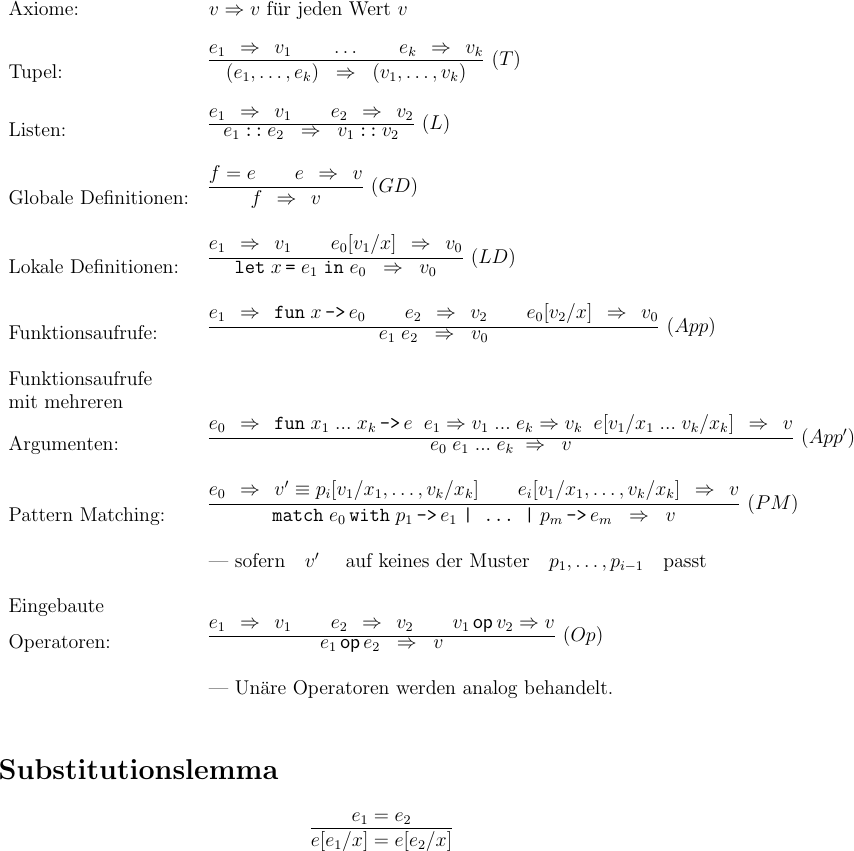
\includegraphics[width=0.8\textwidth]{big_step_rules.png}
	\centering
	\caption{Big-Step-Regeln}\label{big_step_rules}
\end{figure}
\\Da fragt man sich vielleicht zunächst, was dieses ``$\Rightarrow$'' bedeutet und was der Unterschied zu einem ``$=$'' sein soll.
\begin{itemize}
\item \underline{$\Rightarrow$:} Lesen wir $e\Rightarrow v$ für einen Ausdruck e und eine Wert v, so bedeutet dies ``e wertet sich zu v aus''. Ein Wert ist dabei, etwas salopp gesagt, nichts anderes als ein Ausdruck, der nicht weiter durch die oben genannten Regeln vereinfacht werden kann.\\
Beispielsweise können wir $1+2+3\Rightarrow 6$ oder $1\Rightarrow 1$ oder auch $fun\ x \rightarrow x+1\Rightarrow fun\ x \rightarrow x+1$ schreiben. Hingegen ist $fun\ a\ b\rightarrow a+b\Rightarrow fun\ a\ b\rightarrow b+a$ \textbf{nicht} gültig.
\item \underline{$=$:} Lesen wir $e_1=e_2$ für zwei Ausdrücke $e_1$ und $e_2$, so bedeutet dies~-~erneut etwas salopp formuliert~-~``$e_1$ und $e_2$ verhalten sich äquivalent''. Dies bedeutet insbesondere, dass aus $e \Rightarrow v$ sofort $e=v$ folgt.\\
Beispielsweise können wir $1+2+3=6$ oder $fun\ a\ b\rightarrow a+b=fun\ a\ b\rightarrow b+a$ oder \makebox{$(let\ rec\ f\ x=f\ x)\mathbin{\textcolor{red}{=}}(let\ rec\ g\ x\ y=g\ 1\ 2)$} schreiben. Im letzten Beispiel tritt das Gleichheitssymbol sowohl als Definitionsoperator von OCaml (``=''), als auch als Gleichheitssymbol für unsere Big-Step-Semantik (``$\mathbin{\textcolor{red}{=}}$'') auf und die beiden Terme sind äquivalent, da sie beide nicht terminieren und sich somit äquivalent verhalten.
\end{itemize}
\section{Fallbeispiele}
Wie können wir nun das Ganze nutzen, um die Semantik unserer Programme zu überprüfen? Dies sollen die folgenden zwei Beispiele erläutern.
\subsection{Einfacher Ableitungsbaum}
Gegeben sind folgende OCaml-Definitionen
\begin{align*}
	let\ w\ l = match\ l\ with\ []\ \rightarrow 0\ |\ x::xs\ \rightarrow x\\
	let\ r = match\ w\ [1;2]\ with\ 0\ \rightarrow 42\ |\ x\ \rightarrow x+10*2
\end{align*}
Zeigen Sie, dass r=21 gilt.
\begin{proof}
Wir definieren uns zunächst ein paar Kürzel, um den Beweisbaum übersichtlich zu halten
\begin{align*}
	e_0&\coloneqq match\ w\ [1;2]\ with\ 0\ \rightarrow 42\ |\ x\ \rightarrow x+10*2\\
	e_1&\coloneqq match\ l\ with\ []\ \rightarrow 0\ |\ x::xs\ \rightarrow x\\
	f_0&\coloneqq fun\ l\rightarrow e_1
\end{align*}
und beginnen dann von unten den Ableitungsbaum zu zeichnen. Die Anwendung des Axiomes $v\Rightarrow v$ lassen wir zu Gunsten der besseren Übersicht weg.\\
\begin{landscape}
\[
\mkern-50mu
\inferrule* [left=($GD^1$)]
{    
  {r=e_0} 
  \inferrule* [left=($PM^2$)]
  {
	\inferrule*[left=($APP^3$)]
	{
		\inferrule*[left=($GD^4$)]
		{
			{w=f_0}
		}
		{w\Rightarrow f_0}
		\inferrule*[left=($L^5$)]
		{
			\inferrule*[left=($L^6$)] { }
			{[2]\Rightarrow [2]}
		}
		{[1;2]\Rightarrow[1;2]}
		\inferrule*[left=($PM^7$)]
		{
			\inferrule*[left=($L^8$)]
			{
				\inferrule*[left=($L^9$)] { }
				{[2]\Rightarrow [2]}
			}
			{[1;2]\Rightarrow[1;2]\equiv 1::[2]}\\
			{x[1/x]\Rightarrow 1}
		}
		{e_1[[1;2]/l]\Rightarrow 1}
	}
	{w\ [1;2]\Rightarrow 1\equiv x[1/x]}
	\inferrule*[right=($OP^{10}$)]
	{
		\inferrule*[right=($OP^{11}$)]
		{
			{10*2\Rightarrow 20}
		}
		{10*2\Rightarrow 20}\\
		{1+20\Rightarrow 21}
	}
	{1+10*2\Rightarrow 21}
  }
  {e_0\Rightarrow 21}
}
{r\Rightarrow 21}
\]
Im Superskript der angewendeten Regel steht hier jeweils der Zeitpunkt, zu dem die Regel angewandt wurde, um euch den Ablauf klarer zu machen.\\
Im Prinzip schreibt man sich die zu behauptende Aussage unten auf sein Blatt auf und versucht dann bottom-up mit Hilfe der Regeln aus Abb.~\ref{big_step_rules} einen gültigen Ableitungsbaum zu finden. Dabei arbeitet man sich bei jedem Schritt von links nach rechts voran. Wenn man dann einen Wert nach oben berechnet hat, kann man diesen als Ergebnis der Auswertung nach unten einsetzen.
\end{landscape}
\end{proof}

\subsection{Induktion - Terminierung}
Gegeben sind folgende OCaml-Definitionen
\begin{equation*}
	let\ rec\ f\ l = match\ l\ with\ []\ \rightarrow 0\ |\ x::xs\ \rightarrow x+f\ xs
\end{equation*}
Zeigen Sie, dass für alle Integer-Listen l der Aufruf f l terminiert.
\begin{proof}
Wir zeigen die Behauptung mit Induktion.\\
Wie wir auf dem Grundlagenblatt für Induktion gelernt haben, brauchen wir für eine Induktion eine partielle Ordnung $\preceq$, die keine unendlich absteigende Ketten besitzt. Nun lässt sich diese einfach für den Datentyp der Listen festlegen, indem wir für zwei Listen l1 und l2 definieren
\begin{equation*}
	l1\preceq l2:\iff \exists y.\ l2=y@l1
\end{equation*}
Somit können wir vereinfacht ausgedrückt sagen: Wir führen die Induktion über die Länge der Liste \makebox{$n\coloneqq length\ l\in \mathbb{N}_0$}.\\
Wir setzen nun
\begin{align*}
	e_0&\coloneqq match\ l\ with\ []\ \rightarrow 0\ |\ x::xs\ \rightarrow x+f\ xs\\
	f_0&\coloneqq fun\ l\rightarrow e_0
\end{align*}
Die Anwendung des Axiomes $v\Rightarrow v$ lassen wir zu Gunsten der besseren Übersicht weg.
\begin{itemize}
\item \underline{Induktionsbasis:} Sei n=0, dann gilt $l=[]$ und somit
\[
\inferrule*[left=(APP)]{
	\inferrule*[left=(GD)]
	{
		{f=f_0}
	}
	{f\Rightarrow f_0}
	\inferrule*[left=(PM)]
	{
		{[]\Rightarrow[]\equiv[]}\\
		{0\Rightarrow 0}
	}
	{e_0[[]/l]\Rightarrow 0}
}
{f\ []\Rightarrow 0}
\]
Somit terminiert der Basisfall.
\item \underline{Induktionsschritt:} Sei $n\in \mathbb{N}_0$ beliebig fixiert, l eine beliebige Liste mit $n=length\ l$ und $x\in\mathbb{Z}$ beliebig, sodass $n+1=length\ (x::l)$.
	\begin{itemize}
	\item \underline{Induktionshypothese:} Es gelte, dass $f\ l$ terminiert.
	\item \underline{Induktionsbehauptung:} Dann gilt auch, dass $f\ (x::l)$ terminiert.
	\item \underline{Beweis:}
\[
\mkern-100mu
\inferrule*[left=(APP)]{
	\inferrule*[left=(GD)]
	{
		{f=f_0}
	}
	{f\Rightarrow f_0}
	\inferrule*[left=(L)]
	{ }
	{x::l\Rightarrow x::l}
	\inferrule*[right=(PM)]
	{
		{x::l\Rightarrow x::l\equiv x::xs[x/x,l/xs]}\\
		\inferrule*[left=(OP)]
		{
			\inferrule*[left=(I.H.)]{ }
			{f\ l\Rightarrow v}\\
			{x+v\Rightarrow v'}
		}
		{x+f\ l\Rightarrow v'}
	}
	{e_0[(x::l)/l]\Rightarrow v'}
}
{f\ (x::l)\Rightarrow v'}
\]
	\end{itemize}
\end{itemize}
\end{proof}
Grundsätzlich hätten wir auch strenger zeigen können, dass die Funktion f nicht nur terminiert, sondern wirklich die Summe der Zahlen der Liste berechnet. Einfacher und übersichtlicher ist es aber meist, mit Big-Step die Terminierung einer Funktion zu zeigen und anschließend die Semantik des Programmes mit einem gelockerten Formalismus zu beweisen (siehe equivalence\_proofs).
\section{Übungen}
Semester 2016/17
\begin{itemize}
\item Blatt 12
\end{itemize}
GitHub
\begin{itemize}
\item 2016/big\_step
\end{itemize}
Einfach selber Programme schreiben und diese beweisen! :)
\end{sloppypar}
\end{document}
